\documentclass[tikz,border=10pt]{standalone}
\usepackage[T1]{fontenc}
\usepackage{lmodern}
\definecolor{ink}{HTML}{183444}
\definecolor{blue}{HTML}{1B6780}
\definecolor{amber}{HTML}{AD601A}
\begin{document}
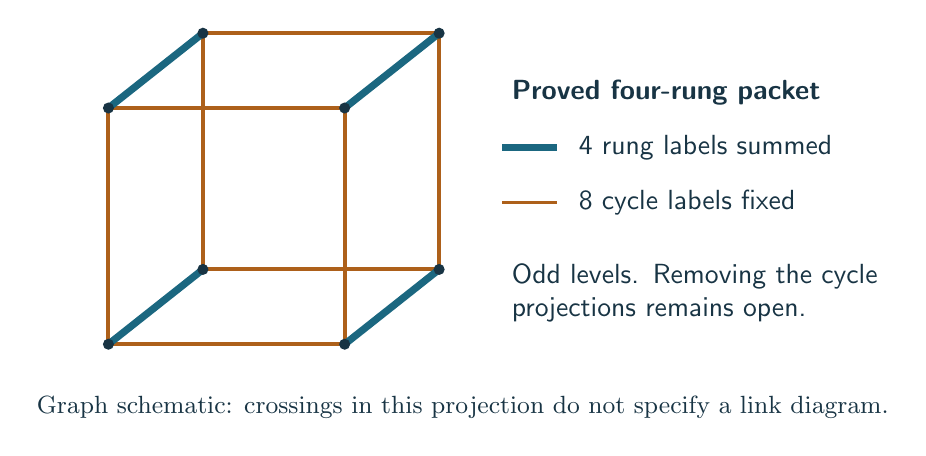
\begin{tikzpicture}[font=\sffamily,text=ink,line join=round]
 \coordinate(a)at(0,0);\coordinate(b)at(3,0);\coordinate(c)at(3,3);\coordinate(d)at(0,3);
 \coordinate(e)at(1.2,.95);\coordinate(f)at(4.2,.95);\coordinate(g)at(4.2,3.95);\coordinate(h)at(1.2,3.95);
 \draw[amber,line width=1.4pt] (a)--(b)--(c)--(d)--cycle;
 \draw[amber,line width=1.4pt] (e)--(f)--(g)--(h)--cycle;
 \foreach \x/\y in {a/e,b/f,c/g,d/h}{\draw[blue,line width=2.6pt](\x)--(\y);}
 \foreach \x in {a,b,c,d,e,f,g,h}{\fill[ink](\x)circle(2pt);}
 \node[anchor=west]at(5,3.2){\textbf{Proved four-rung packet}};
 \draw[blue,line width=2.6pt](5,2.5)--(5.7,2.5);\node[anchor=west]at(5.85,2.5){4 rung labels summed};
 \draw[amber,line width=1.4pt](5,1.8)--(5.7,1.8);\node[anchor=west]at(5.85,1.8){8 cycle labels fixed};
 \node[anchor=west,text width=4.7cm,align=left]at(5,.65){Odd levels. Removing the cycle projections remains open.};
 \node[font=\small]at(4.5,-.8){Graph schematic: crossings in this projection do not specify a link diagram.};
\end{tikzpicture}
\end{document}
